% ==============================================================================
% =================================== Aufgabe 3 =================================
% ==============================================================================

\chapter{Aufgabe}
\label{chap:3 Aufgabe}
\thispagestyle{fancy}
\section*{} 
\begin{figure}[h]
    \centering
    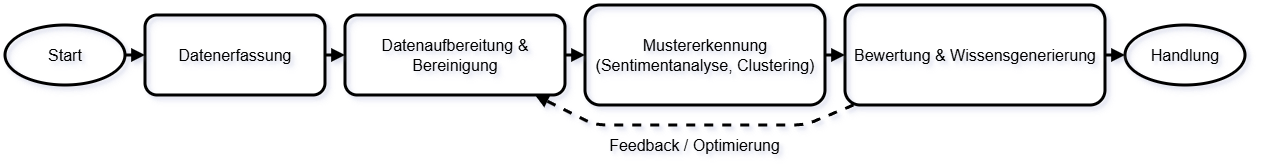
\includegraphics[width=0.95\textwidth]{./asset/image/Data-Mining-Prozess.png}
    \caption{Data-Mining-Prozess für Internettexte}
    \label{fig:dataminingprozess}
    [Quelle: Eigene Darstellung]
\end{figure}
Gattnar \cite[25]{18} charakterisiert den \uline{Data-Mining-Prozess} grundlegend als eine automatisierte Suche nach Mustern, Regeln und Abhängigkeiten in großen Datenbeständen, mit dem Ziel, handlungsrelevantes Wissen zu generieren. Im Kontext von \uline{Internettexten} (\textit{\acs{z. B.} aus Foren, Blogs oder sozialen Medien}) kommt dabei häufig das \uline{Text-Mining} zum Einsatz, um unstrukturierte Daten automatisiert zu erfassen und sinnvoll zuzuordnen. \par Hinsichtlich der Verarbeitung von Internettexten durchläuft der \uline{Data-Mining-Prozess}, wie in der folgenden \hyperref[fig:dataminingprozess]{Abbildung \ref{fig:dataminingprozess}} visualisiert, folgende vier wesentliche, aufeinander aufbauende Phasen:
\begin{enumerate}[label=\arabic*.), leftmargin=*]
    \item \textbf{Datenerfassung (\textit{Extraktion}):} Das Unternehmen sammelt Texte aus externen Quellen wie \uline{Internetforen (\textit{\acs{z. B.} motor-talk.de})}, \uline{Blogs} oder \uline{sozialen Netzwerken}. Ein konkretes Beispiel, so wie Gronau \cite[124]{19} im Kontext des analytischen \acs{CRM} darlegt, ist die Aufbereitung unstrukturierter Daten für ein Customer Data Warehouse eine zwingende Voraussetzung, um externes Kundenfeedback etwa nach einem Produktlaunch systematisch nutzbar zu machen.
    \item \textbf{Datenaufbereitung und Bereinigung:} Internettexte sind oft durch Dialekte, Slang, Sarkasmus oder Rechtschreibfehler geprägt. Im Rahmen der Datenveredelung müssen diese Hindernisse überwunden werden, um eine \uline{semantische Harmonisierung} zu erreichen. Abkürzungen müssen korrekt interpretiert werden, um Fehlinterpretationen in der späteren Analyse zu vermeiden.
    \item \textbf{Mustererkennung (\textit{Eigentliches Mining}):} In ihrer systematischen Darstellung der Business Intelligence hebt Goram \cite[48]{20} hervor, dass in dieser Phase gezielt Algorithmen eingesetzt werden, um tiefergehende Bedeutungen aus den zuvor aufbereiteten Texten abzuleiten.
    \begin{itemize}
        \item \textbf{Sentimentanalyse:} Ein häufiges Verfahren ist die Analyse des „Meinungsbildes“. Hierbei wird automatisch bestimmt, ob ein Text (\textit{\acs{z. B.} ein Tweet oder Forenbeitrag}) eine \uline{positive}, \uline{negative} oder \uline{neutrale Stimmung} gegenüber einem Produkt ausdrückt. Dies geschieht entweder durch Machine-Learning-Ansätze oder wörterbuchbasierte Verfahren.
        \item \textbf{Clustering:} Texte mit ähnlichen Inhalten oder Stimmungen können gruppiert werden, um homogene Kundensegmente zu entdecken.
    \end{itemize}
    \item \textbf{Bewertung und Wissensgenerierung:} Die gefundenen Muster werden in handlungsorientiertes Wissen transformiert.
    \begin{itemize}
        \item \textbf{Beispiel:} Erkennt das System durch Data Mining eine Häufung negativer Begriffe im Zusammenhang mit einem bestimmten Bauteil in Internetforen, kann das Unternehmen frühzeitig reagieren, bevor offizielle Reklamationen massiv zunehmen.
        \item \textbf{Rückgewinnungsanalyse:} Durch die Analyse der Texte können abwanderungswillige Kunden identifiziert werden, um ihnen gezielte Angebote zur Erhaltung ihrer Loyalität zu machen.
    \end{itemize}
\end{enumerate}
Zusammenfassend dient Data Mining bei Internettexten dazu, das \uline{Kundenverhalten} und \uline{die Marktposition besser zu verstehen}, indem aus einer Flut unstrukturierter Texte gezielt verwertbare Informationen extrahiert werden.

% ==============================================================================
% =================================== Aufgabe 3 =================================
% ==============================================================================